% Mirror: https://github.com/SIGma-UIUC/presentation-format
% --------------------------------------------------------------------
% This is a simple Beamer document that uses beamerthemesigma.sty
% Reading the comments should help you create a presentation even if
% you've never used Beamer before.
% --------------------------------------------------------------------

% Set our document class to Beamer
\documentclass[aspectratio=169]{beamer}
% \documentclass[aspectratio=169, handout]{beamer}
% Add handout option to ignore pauses

% From Jeff E
\usepackage{algo}
% Some more macros
\usepackage{sigmastyle}

\usepackage{colortbl}
\definecolor{LightRed}{RGB}{252,160,140}
\newcolumntype{a}{>{\columncolor{LightRed}}c}


% Set a title
\title{Linear and Cyclic Codes}

% Set a subtitle if you desire
\subtitle{}

% Whoever worked on the presentation:
\author{Hassam}

% Date looks ugly, so leave blank
\date{}

% An institute name, if you're so inclined
% \institute{University of Illinois Urbana-Champaign}

% Use the SIGma theme for this Beamer presentation
\usetheme{sigma}
% --------------------------------------------------------------------


\newcommand{\err}[1]{{\color{sigma@alertred}#1}}
\newcommand{\blu}[1]{{\color{sigma@mainblue}#1}}
% Begin document
\begin{document}

% Beamer calls each slide a "frame", defined within the environment:
% \begin{frame}
%   <frame content here>
% \end{frame}

% This frame is just the title.
\begin{frame}
\titlepage
\end{frame}


\begin{frame}{The Basic Problem (revisited)}
    \begin{itemize}
        \item Sending messages between parties might be subject to errors.
        \item How do we:
            \begin{itemize}
                \item Detect Errors? 
                \item Correct Errors?
            \end{itemize}
        \item The goal is to send a message that minimizes the necessary redundancy to achieve both goals. 
        \item What if we only care about certain common types of errors? 
    \end{itemize}
\end{frame}

\section{Mathing up Hamming Codes}
\frame{\sectionpage}

\begin{frame}{Reminder of Hamming Codes}
    \begin{itemize}
        \item We can detect the error by checking each parity bit, and fix it!
    \end{itemize}
    \begin{columns}[c]
    \begin{column}{2cm}
    \begin{table}
        \centering
        \begin{tabular}{|c|a|c|a|}
            \hline 
            0 & 1 & 1 & 0 \\ \hline
            1 & 1 & \blu{0} & 0 \\ \hline
            0 & 1 & 0 & 0 \\ \hline
            1 & 0 & 1 & 1 \\ \hline
        \end{tabular}
    \end{table}
    \end{column}
    \hfill
    \begin{column}{2cm}
    \begin{table}
        \centering
        \begin{tabular}{|c|c|a|a|}
            \hline 
            0 & 1 & 1 & 0 \\ \hline
            1 & 1 & \blu{0} & 0 \\ \hline
            0 & 1 & 0 & 0 \\ \hline
            1 & 0 & 1 & 1 \\ \hline
        \end{tabular}
    \end{table}
    \end{column}
    \hfill
    \begin{column}{2cm}
    \begin{table}
        \centering
        \begin{tabular}{|c|c|c|c|}
            \hline 
            0 & 1 & 1 & 0 \\ \hline
            \rowcolor{LightRed}
            1 & 1 & \blu{0} & 0 \\ \hline
            0 & 1 & 0 & 0 \\ \hline
            \rowcolor{LightRed}
            1 & 0 & 1 & 1 \\ \hline
        \end{tabular}
    \end{table}
    \end{column}
    \hfill
    \begin{column}{2cm}
    \begin{table}
        \centering
        \begin{tabular}{|c|c|c|c|}
            \hline     
            0 & 1 & 1 & 0 \\ \hline
            1 & 1 & \blu{0} & 0 \\ \hline
            \rowcolor{LightRed}
            0 & 1 & 0 & 0 \\ \hline
            \rowcolor{LightRed}
            1 & 0 & 1 & 1 \\ \hline
        \end{tabular}
    \end{table}
    \end{column}
    \end{columns}
\end{frame}

\begin{frame}{Going Higher}
    \begin{itemize}
        \item What does it really mean to correct an error? 
        \item Let's consider a simple code: ``best 2 out of 3''. 
        \item Encode message $m$ by taking each bit and repeating it three times. \pause
        \item Our valid ``words'': $000$ and $111$, but the language contains $2^3$ words. 
        \item We are raising the dimension of our message space, giving us more room to detect errors. 
    \end{itemize}
\end{frame}

\begin{frame}{Going Higher}
    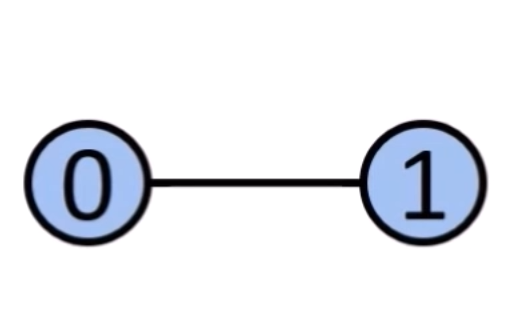
\includegraphics[width=0.4\textwidth]{images/01.png}
    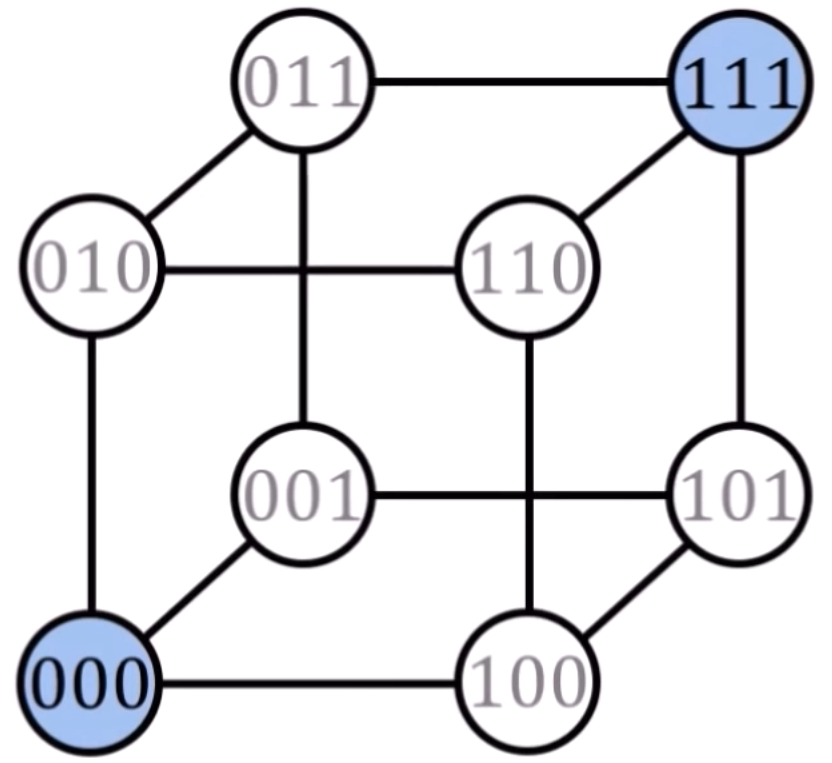
\includegraphics[width=0.4\textwidth]{images/000-111.png}
\end{frame}

\begin{frame}{Hamming (7, 4) (because the dimensions are smaller)}
    \begin{itemize}
        \item \emph{$(n, k)$ code} means $n$ bits to encode a $k$ bit message. \pause 
        \item Consider a message with 4 bits. We can use 3 additional bits of information to ``search'' over these bits and detect errors, just like the earlier Hamming example. \pause 
        \item $p_0 = m_0 + m_1 + m_3$, $p_1 = m_0 + m_2 + m_3$, $p_2 = m_1 + m_2 + m_3$. All $\mod 2$.
        \item  Convince yourself that we can detect, and find, any 1-bit error using these check bits. 
    \end{itemize}
\end{frame}

\begin{frame}{Linear Equations $\implies$ Linear Algebra}
    Can we create a matrix $G$ that converts our message into a code? $mG = c$ \pause

 \begin{gather*}
 mG = \begin{bmatrix}
        m_0 & m_1 & m_2 & m_3
  \end{bmatrix} \begin{bmatrix}
      1 & 0 & 0 & 0 & 1 & 1 & 0 \\
      0 & 1 & 0 & 0 & 1 & 0 & 1 \\
      0 & 0 & 1 & 0 & 0 & 1 & 1 \\
      0 & 0 & 0 & 1 & 1 & 1 & 1
  \end{bmatrix} = \\ 
  \begin{bmatrix}
      m_0 & m_1 & m_2 & m_3 & m_0 + m_1 + m_3 & m_0 + m_2 + m_3 & m_1 + m_2 + m_3
  \end{bmatrix} = \\
  \begin{bmatrix}
      m_0 & m_1 & m_2 & m_3 & p_0 & p_1 & p_2
  \end{bmatrix} = c
  \end{gather*}
\end{frame}

\begin{frame}{Linear Algebra $\implies$ ?}
    \begin{itemize}
        \item Turning Hamming Codes into a matrix gives us linearity for free! \pause
        \item Namely, the sum of any two messages is a valid message, and, by linearity, the sum of any two codewords is also a codeword. \pause 
        \item Let's see if we can prove some nice properties using this. 
    \end{itemize}
\end{frame}

\begin{frame}{Minimum Distance (revisited)}
    \begin{itemize}
        \item The \emph{Minimum Distance} of a code is the minimum difference between any two codewords. 
        \begin{itemize}
            \item $\Delta(x, y)$ is the number of positions $i$ where characters $x[i] \neq y[i]$ 
        \end{itemize} \pause
        \item More formally $\min\limits_{c_1, c_2} \Delta(c_1, c_2)$ \pause
        \item But this is just $\min\limits_{c_1, c_2} \Delta(0, c_2 - c_1)$ \pause 
        \item But again, this is just $\min\limits_{c} \Delta(0, c)$ = $\min\limits_c w(c)$
    \end{itemize}
\end{frame}

\begin{frame}{Parity Checking (but with linear algebra this time)}
    \begin{itemize}
        \item Can we find a matrix, $H$, such that $Hc^T = 0$. \pause Why? \pause
        \item Linearity! 
        \item Suppose we transmitted some code $c$ with error $e$, $c + e$, then: $H(c + e)^T = Hc^T + He^T = He^T$. What is $He^T$? \pause 
        \item It is the column in $H$ associated with the error \pause 
        \item Since we know where in $H$ the error is, we know which bit of the message it corresponds to. We can both detect errors and correct them! We call this the ``syndrome'' vector. \pause 
        \item $HG^T = 0$ and so it follows that $H = \begin{bmatrix}P | I_{n - k} \end{bmatrix}$. Verify this yourself. 
    \end{itemize}
\end{frame}

\begin{frame}{Generalizing Hamming Codes}
    \begin{itemize}
        \item Hamming codes are a code such that the Parity-Check matrix has columns with every possible combination of 0s and 1s, except for all 0s. \pause 
        \item So to make a Hamming code for higher dimensions, create a matrix of every single binary number, rotate them so that the identity is in the last columns, and the remaining columns are our parity checks. 
    \end{itemize}
\end{frame}

\setcounter{MaxMatrixCols}{20}
\begin{frame}{Generalizing Hamming Codes}
    $$\begin{bmatrix}
        1 & 0 & 1 & 0 & 1 & 0 & 1 & 0 & 1 & 0 & 1 & 0 & 1 & 0 & 1 \\
        0 & 1 & 1 & 0 & 0 & 1 & 1 & 0 & 0 & 1 & 1 & 0 & 0 & 1 & 1 \\
        0 & 0 & 0 & 1 & 1 & 1 & 1 & 0 & 0 & 0 & 0 & 1 & 1 & 1 & 1 \\
        0 & 0 & 0 & 0 & 0 & 0 & 0 & 1 & 1 & 1 & 1 & 1 & 1 & 1 & 1
    \end{bmatrix}$$
\end{frame}

\begin{frame}{Generalizing Hamming Codes}
    Moving the previous columns around to form a parity check matrix then gives into: 
    $$\begin{bmatrix}
        0 & 1 & 1 & 0 & 1 & 0 & 1 & 1 & 1 & 0 & 1 & | & 1 & 0 & 0 & 0 \\
        0 & 0 & 1 & 1 & 0 & 1 & 1 & 1 & 0 & 1 & 1 & | & 0 & 1 & 0 & 0 \\
        1 & 1 & 0 & 1 & 1 & 1 & 1 & 1 & 0 & 0 & 0 & | & 0 & 0 & 1 & 0 \\
        1 & 1 & 0 & 1 & 0 & 0 & 0 & 1 & 1 & 1 & 1 & | & 0 & 0 & 0 & 1
    \end{bmatrix}$$

    Each row covers one bit of the message, together covering them all. 
\end{frame}

\section{Cyclic Codes}
\frame{\sectionpage}

\begin{frame}{Motivation}
    \begin{itemize}
        \item More math! \pause 
        \item Most errors occur in ``bursts''. You might have 5 errors in a message, but they will generally all be concentrated near each other. \pause 
        \item Working under this constraint, rather than detecting arbitrary errors, can give us a lot more power. 
    \end{itemize}
\end{frame}

\begin{frame}{Cyclic}
\begin{itemize}
    \item \emph{Cyclic codes} are relatively self explanatory. \pause 
    \item $C$ is cyclic if $(c_1, c_2, c_3, \ldots, c_n) \in C \implies (c_n, c_1, c_2, \ldots, c_{n - 1}) \in C$. \pause 
    \item Cyclic codes by themselves are not really useful
\end{itemize}
\end{frame}

\begin{frame}{(Linear) Cyclic}
\begin{itemize}
    \item A much more useful and practical type of codespace is one where every codeword is cyclic AND linear. 
    \item Example codespace: $000000$, $100100$, $010010$, $001001$, $110110$, $011011$, $101101$, $111111$. \pause
    \item Every codeword can be written as the sum of two other codewords, and every sum of codewords is a codeword. Similarly, shifting any codeword will produce a valid codeword. 
\end{itemize}
\end{frame}

\begin{frame}{Polynomials (an aside)}
    \begin{itemize}
        \item We can think of these codewords as a sequence, and create a polynomial called a \emph{generating function}. For example: $100100 = 1x^0 + 0x^1 + 0x^2 + 1x^3 + 0x^4 + 0x^5 = 1 + x^3$. \pause
        \item Polynomials have a lot of nice properties similar to the integers. 
        \item Namely, we can do polynomial division, and modular arithmetic over polynomials. We will often write $\Z_2[x]$ to talk about polynomials with $\{0, 1\}$ as the coefficients. 
    \end{itemize}
\end{frame}

\begin{frame}{Modular Arithmetic with Polynomials}
    \begin{itemize}
        \item Consider $(x^3 + x^2 + 1) / (x^2 + 1) = (x^2 + 1)q(x) + r(x)$.  
        \begin{itemize}
            \item What are $q(x)$ and $r(x)$ if our polynomial is in $\Z_2[x]$? \pause
            \item $q = x + 1$, $r = -x = x$.
        \end{itemize}
        \item So, $x^3 + x^2 + 1 \equiv x \mod (x^2 + 1)$. \pause 
        \item We will primarily work mod polynomials of the form $f(x) \pm 1$
        \begin{itemize}
            \item So $f(x) \pm 1$ acts like $0$
            \item You can think of substituting every occurrence of $f(x)$ with $1$. 
        \end{itemize}
    \end{itemize}
\end{frame}

\begin{frame}{Cyclic Codes fall out naturally}
    \begin{itemize}
        \item Let's go back to one of our initial codewords: $100100 \equiv 1 + x^3$. \pause 
        \item The maximum degree of a polynomial in this codespace is $x^5$
        \item If we take our codewords mod $x^6 + 1$, then $x \cdot (1 + x^3) = x + x^4 \equiv 010010$, which is another codeword. \pause 
        \item  We can continue to shift our codewords by multiplying by $x$, and if we go over $x^5$, our modulo wraps it back around! So, $c(x) \in C \implies x c(x) \in C$. 
    \end{itemize}
\end{frame}

\begin{frame}{Linearity strikes back}
    Recall that our codewords are not just cyclic, but also linear. So, if $c(x) \in C$, then $c(x) + c(x) \in C$. \pause
    
    Since $x^nc(x) \in C$, this means that $(1 + x + x^2 + \ldots) c(x) \in C$. In otherwords, for any polynomial, $g(x)$, then $g(x)c(x) \in C$. 
\end{frame}

\begin{frame}{Generator Polynomial}
    If we can make other valid codewords using any polynomial, we just need 1 codeword to ``generate'' the rest. (I apologize for the differing uses of generate, blame whoever came up with this stuff). \pause 

    Consider again: $000000$, $100100$, $010010$, $001001$, $110110$, $011011$, $101101$, $111111$. Can we generate all of the other codewords from $100100$, or $g(x) = 1 + x^3$, mod $x^6 + 1$? 
\end{frame}

\begin{frame}{Generator Polynomial}
    \begin{align*}
    0 &= 0 \cdot g(x) \\
    1 + x^3 &= 1 \cdot g(x) \\ 
    x + x^4 &= xg(x) \\
    x^2 + x^5 &= x^2g(x) 
    \end{align*} \pause
    \begin{align*}
    1 + x + x^3 + x^4 &= (1 + x)g(x) \\ 
    x + x^2 + x^4 + x^5 &= (x + x^2)g(x) \\
    1 + x^2 + x^3 + x^5 &= (1 + x^2)g(x) 
    \end{align*}
    
    and $1 + x + x^2 + x^3 + x^4 + x^5 = (1 + x + x^2)g(x)$. Is the generator polynomial within a codespace unique? 
\end{frame}

\begin{frame}{Generator Polynomial}
    \begin{itemize}
        \item No it is not! 
        \item We could have used any of the first three codewords and shifted things accordingly, but in general, we call the polynomial with the lowest degree the generator polynomial. \pause 
        \item We can encode a message of size $k$ using a generator polynomial with max degree $r = n - k$, $c(x) = m(x)g(x)$. \pause 
        \item Since these are linear codes, we can create a generator matrix just like we did for linear codes. 
        \item These are not super interesting, so I'll leave it up to you all to think about how to form them. 
    \end{itemize}
\end{frame}

\begin{frame}{Correcting}
    \begin{itemize}
        \item Briefly, if $c(x) = m(x)g(x)$, we can do $m(x) = c(x)/g(x)$ to get back our original message, if there were no errors. 
        \item If there was an error, we'll have a remainder. For single-bit errors, just like our linear codes, we can create a table of remainders and match our remainder to figure out where the error occurred. 
        \item But, this is no better than Hamming Codes.
    \end{itemize}
     
\end{frame}

\begin{frame}{Cyclic Redundancy Checks}
    We said earlier that cyclic codes can be used to detect burst errors. How? \pause Let's consider this simple scheme, commonly used in networking, known as the \emph{Cyclic Redundancy Check}. 

    \begin{itemize}
        \item Take our message $m(x)$, and multiply it by $x^r$, where $r$ is the degree of our generator polynomial for our codespace, and then divide it by our generator $g(x)$. \pause
        \item We will end up with $x^rm(x) = Q(x)g(x) + R(x)$. \pause
        \item Under $\Z_2$, addition and subtraction are the same operation $\implies Q(x)g(x) = x^r m(x) - R(x) = x^r m(x) + R(x)$.
        \item If we transmit $T(x) = x^rm(x) + R(x)$, this will be divisible by $g(x)$. 
    \end{itemize}
\end{frame}

\begin{frame}{Cyclic Redundancy Checks $\stackrel{?}{=}$ Parity Bits}
    \begin{itemize}
        \item We will only miss errors if they are divisible by $g(x)$, so we could select a $g(x)$ such that it is not divisible by ``common'' things. \pause 
        \begin{itemize}
            \item Indeed, this is how most modern tooling using CRC does it. But let's not rely on that. \pause 
        \end{itemize}
        \item Suppose we transmit $T'(x)$, where $T'$ has some error that causes an odd number of flipped bits. \pause
        \item  Assuming that our initial message has an even number of $1$s, if we've flipped an odd number of bits, then $T'(1) = 1$.
        \item So, as long as $g(1) = 0$, we will detect any odd number of bit flips. Picking $g(x) = x^i + 1$ will always ensure that $g(1) = 0$. \pause 
    \end{itemize} 

    In fact, $g(x) = x + 1$ is equivalent to a parity check bit.  
\end{frame}

\begin{frame}{Cyclic Redundancy Checks}
    \begin{itemize}
        \item So, we can detect any number of odd bit flips, just like a parity bit. What else can we do? 
        \item Suppose we had a sequence of errors in a row. 
        \item Let $E(x) = T(x) - T'(x)$ be which bits are flipped. \pause
        \item $g(x)$ divides $T(x)$ 
        \begin{itemize}
            \item $E(x)$ doesn't divide $T(x) \implies g(x)$ doesn't divide $T'(x)$.
        \end{itemize}
    \end{itemize} \pause

    What does $E(x)$ look like if we had a sequence of $r$ errors? \pause 

    $E(x) = x^{n_1} + x^{n_2} + \ldots + x^{n_r}$, where $n_i$ is a decreasing sequence. 
\end{frame}

\begin{frame}{Math Magic}
    \begin{itemize}
        \item So, we can factor $E(x) = x^{n_r}(x^{n_1 - n_r} + x^{n_2 - n_4} + \ldots + 1)$. \pause 
        \item $g(x) = x^i + 1$ cannot divide $x^{n_r}$. So, CRC can only fail if $g(x)$ divides $x^{n_1 - n_r} + x^{n_2 - n_r} + \ldots + 1$. How can we ensure that never happens? \pause 
        \item Choose $g(x)$ such that it's degree is larger than the number of errors you'd like to detect.
    \end{itemize}


 
\end{frame}

\begin{frame}{Is it worth the effort?}
    \begin{itemize}
        \item Dividing polynomials is hard. I don't want to do it. \pause
        \item The computer is more than happy to do it for you. Dividing polynomials over $\Z_2$ is just a problem of shifting bits and XORing them. \pause
        \item CRC is fast at detecting and correcting errors of size 1, but it's true power shines in detecting any size of burst errors. \pause
    \end{itemize}

    CRC is being used by every single device on the planet when it communicates over the internet. CRC is used the data layer and the transport layer of all computer networks. Sometime soon, we'll discuss more advanced codes (Reed-Solomon) that are used for a lot of other things you're familiar with, like barcodes and QR codes. 
\end{frame}

% Quotes are fun, find some to use!
\font\eightss=cmssq8
\font\eightssi=cmssqi8
\newcommand\quoteAuthorDate[3]{\begingroup
  \baselineskip 10pt
  \parfillskip 0pt
  \interlinepenalty 10000 % not needed in example
  \leftskip 0pt plus 40pc minus \parindent
  \let\rm=\eightss
  \let\sl=\eightssi
  \everypar{\sl}#1\par
  \nobreak\smallskip
  \noindent\rm--- #2\unskip\enspace(#3)\par
  \endgroup}
% If someone can figure out how to horizontally center this and make the text bigger that'd be cool
\begin{frame}
    \begin{center}
        \item \quoteAuthorDate{The field of 'information theory' began by using the old hardware paradigm of transportation of data from point to point.}{MARSHALL MCLUHAN}{\color{sigma@mainblue} 1988}
    \end{center}
\end{frame}

\end{document}